\chapter{Example Chapter}

\Glspl{star} spend most of their life on the \acrfull{ms}. The \acrshort{ms} was discovered when the \gls{luminosity} of many stars were plot against their spectral class. We can see this in Figure \ref{fig:example}. 

\begin{figure}[t]
  \centering
  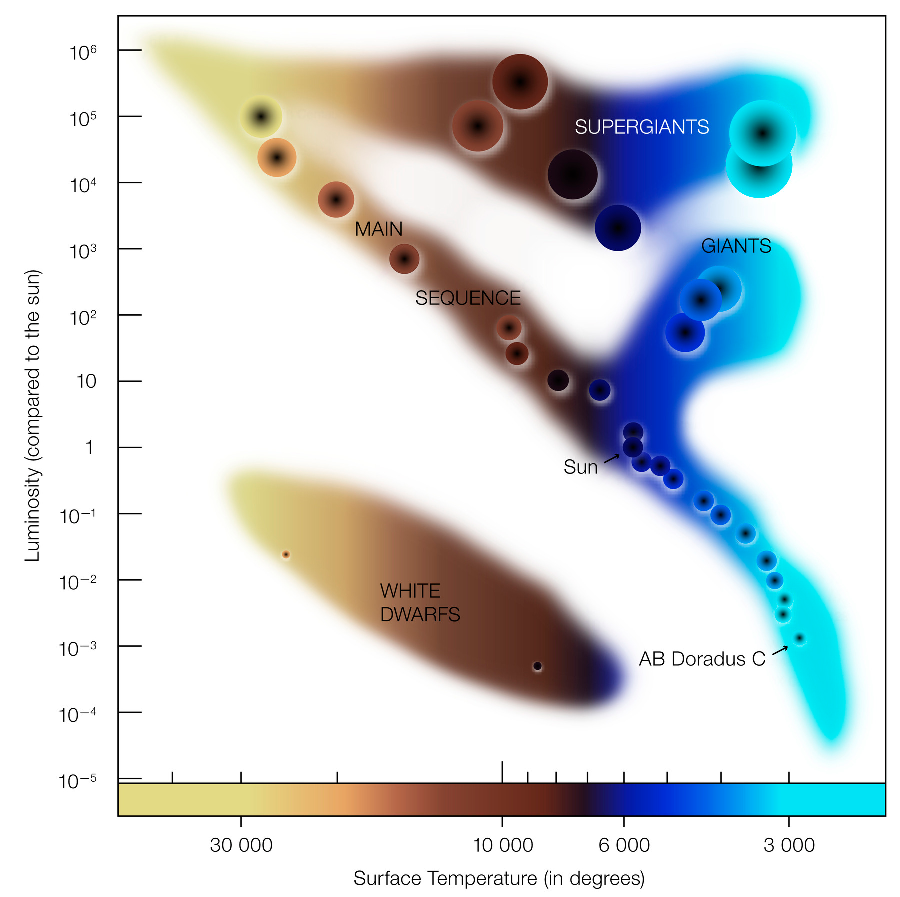
\includegraphics{figures/example.pdf}
  \caption[Short version of caption]{A negative colour version of the Hertzsprung-Russell diagram produced by the European Southern Observatory. \emph{Credit:} \href{https://www.eso.org/public/images/eso0728c/}{ESO}.}
  \label{fig:example}
\end{figure}

Here is an example citation in parentheses \citep{einstein} or we can just refer to \citet{dirac} in text.

\lipsum[17-18]
